\section{Organisation et Planification}

\begin{frame}{Organiser une plongée en autonomie}
    Le N3 peut plonger sans Directeur de Plongée (DP). Il est responsable de l'organisation.
    
    \textbf{Les étapes clés :}
    \begin{enumerate}
        \item Vérifier la \textbf{Météo} (Vents, Houle, Météo France, Apps, CROSS).
        \item Choisir le \textbf{Site} (Profil, niveau des plongeurs, zones interdites).
        \item Préparer le \textbf{Bateau} (Carburant, Mouillage, VHF testée).
        \item Établir la \textbf{Fiche de Sécurité} (Palanquées, paramètres prévus).
    \end{enumerate}
\end{frame}

\begin{frame}{La Météo — Sources d'Information}
    Il existe plusieurs moyens de vérifier la météo avant le départ :
    
    \begin{itemize}
        \item \textbf{Internet} : Sites web spécialisés (Météo France, Lamma, etc.).
        \item \textbf{Applications} : Sur smartphone (Windy, Maree.info, etc.).
        \item \textbf{Capitainerie} : Affichages au port ou renseignement direct.
        \item \textbf{Message Radio du CROSS} (VHF) :
        \begin{itemize}
            \item Se renseigner sur les \textbf{horaires} de diffusion.
            \item Connaître les \textbf{canaux} de diffusion (VHF).
        \end{itemize}
    \end{itemize}
    \centering
    
\includegraphics[height=0.25\textheight, keepaspectratio]{images/meteo} 
\end{frame}

\begin{frame}{Le Choix du Site de Plongée}
    \textbf{Le site se choisit en fonction :}
    \begin{itemize}
        \item Des \textbf{conditions météo}.
        \item Du \textbf{profil} (profondeur, courant potentiel...).
        \item Des \textbf{envies} et de l'\textbf{état physique} des plongeurs.
    \end{itemize}
    
    \vspace{0.8em}
    \textbf{Points de vigilance :}
    \begin{itemize}
        \item Faire attention aux \textbf{zones interdites} (réserves, zones militaires...) indiquées sur les \textbf{cartes marines}.
        \item \textbf{Informer une personne à terre} du lieu choisi et des horaires prévus avant le départ (pour déclencher les secours en cas de retard anormal).
    \end{itemize}
\end{frame}

\begin{frame}{Matériel de Sécurité Obligatoire (Bateau)}
    En tant que responsable, vérifier la présence du matériel (Art. A.322-78-2):
    \begin{columns}[totalwidth=\textwidth]
        \column{0.5\textwidth}
        \textbf{Secours \& Médical :}
        \begin{itemize}
            \item Trousse de secours complète.
            \item Oxygénothérapie (Bavu + O2).
            \item Eau douce potable.
            \item Couverture isothermique.
            \item Fiches d'évacuation.
        \end{itemize}

        \textbf{Opérationnel \& Signalisation :}
        \begin{itemize}
            \item Moyen de communication (VHF).
            \item Bouteille de secours (détendeur monté).
            \item Tables de plongée (immergables).
            \item \textbf{Pavillon Alpha}.
        \end{itemize}
        \vspace{0.5em}
        \column{0.5\textwidth}
        \centering
        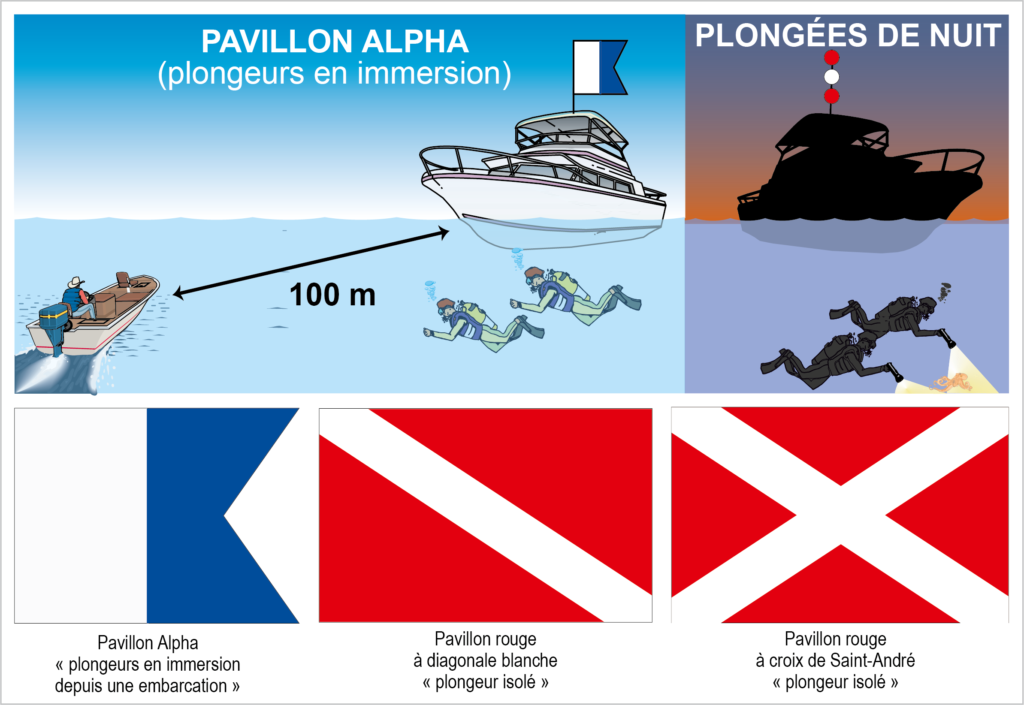
\includegraphics[width=0.9\columnwidth, keepaspectratio]{images/signalisation-plongeurs.png}
    \end{columns}
\end{frame}

\begin{frame}{Procédures d'Urgence — Alerte}
    \textbf{Alerte (CROSS - VHF Canal 16 ou Tél 196)} :
    \begin{itemize}
        \item Message \textbf{PAN-PAN} (Urgence relative) ou \textbf{MAYDAY} (Détresse vitale).
        \item Donner dans l'ordre :
        \begin{enumerate}
            \item \textbf{Position} du navire.
            \item \textbf{Nature} du problème (ADD, Noyade...).
            \item \textbf{Nombre} et état des victimes.
        \end{enumerate}
    \end{itemize}
\end{frame}

\begin{frame}{Plan de Secours}
    \centering
    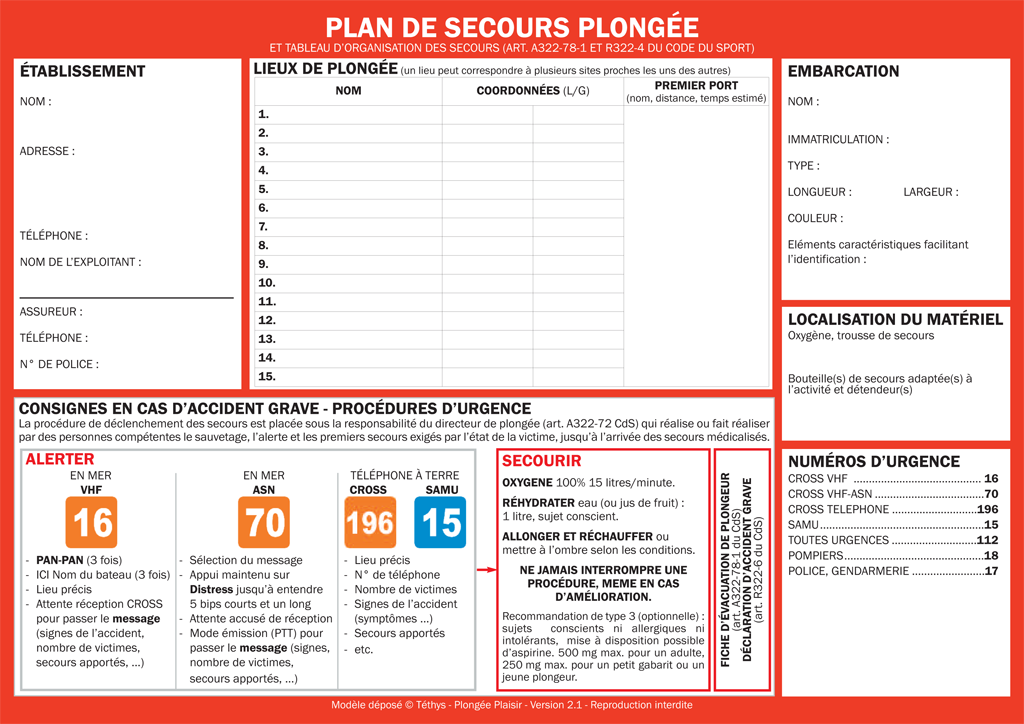
\includegraphics[width=\textwidth, height=0.87\textheight, keepaspectratio]{images/plongee_plaisir_plan_secours.png}
\end{frame}

\begin{frame}{Fiche d'Évacuation}
    \centering
    % Plan d'organisation ou cartographie large
    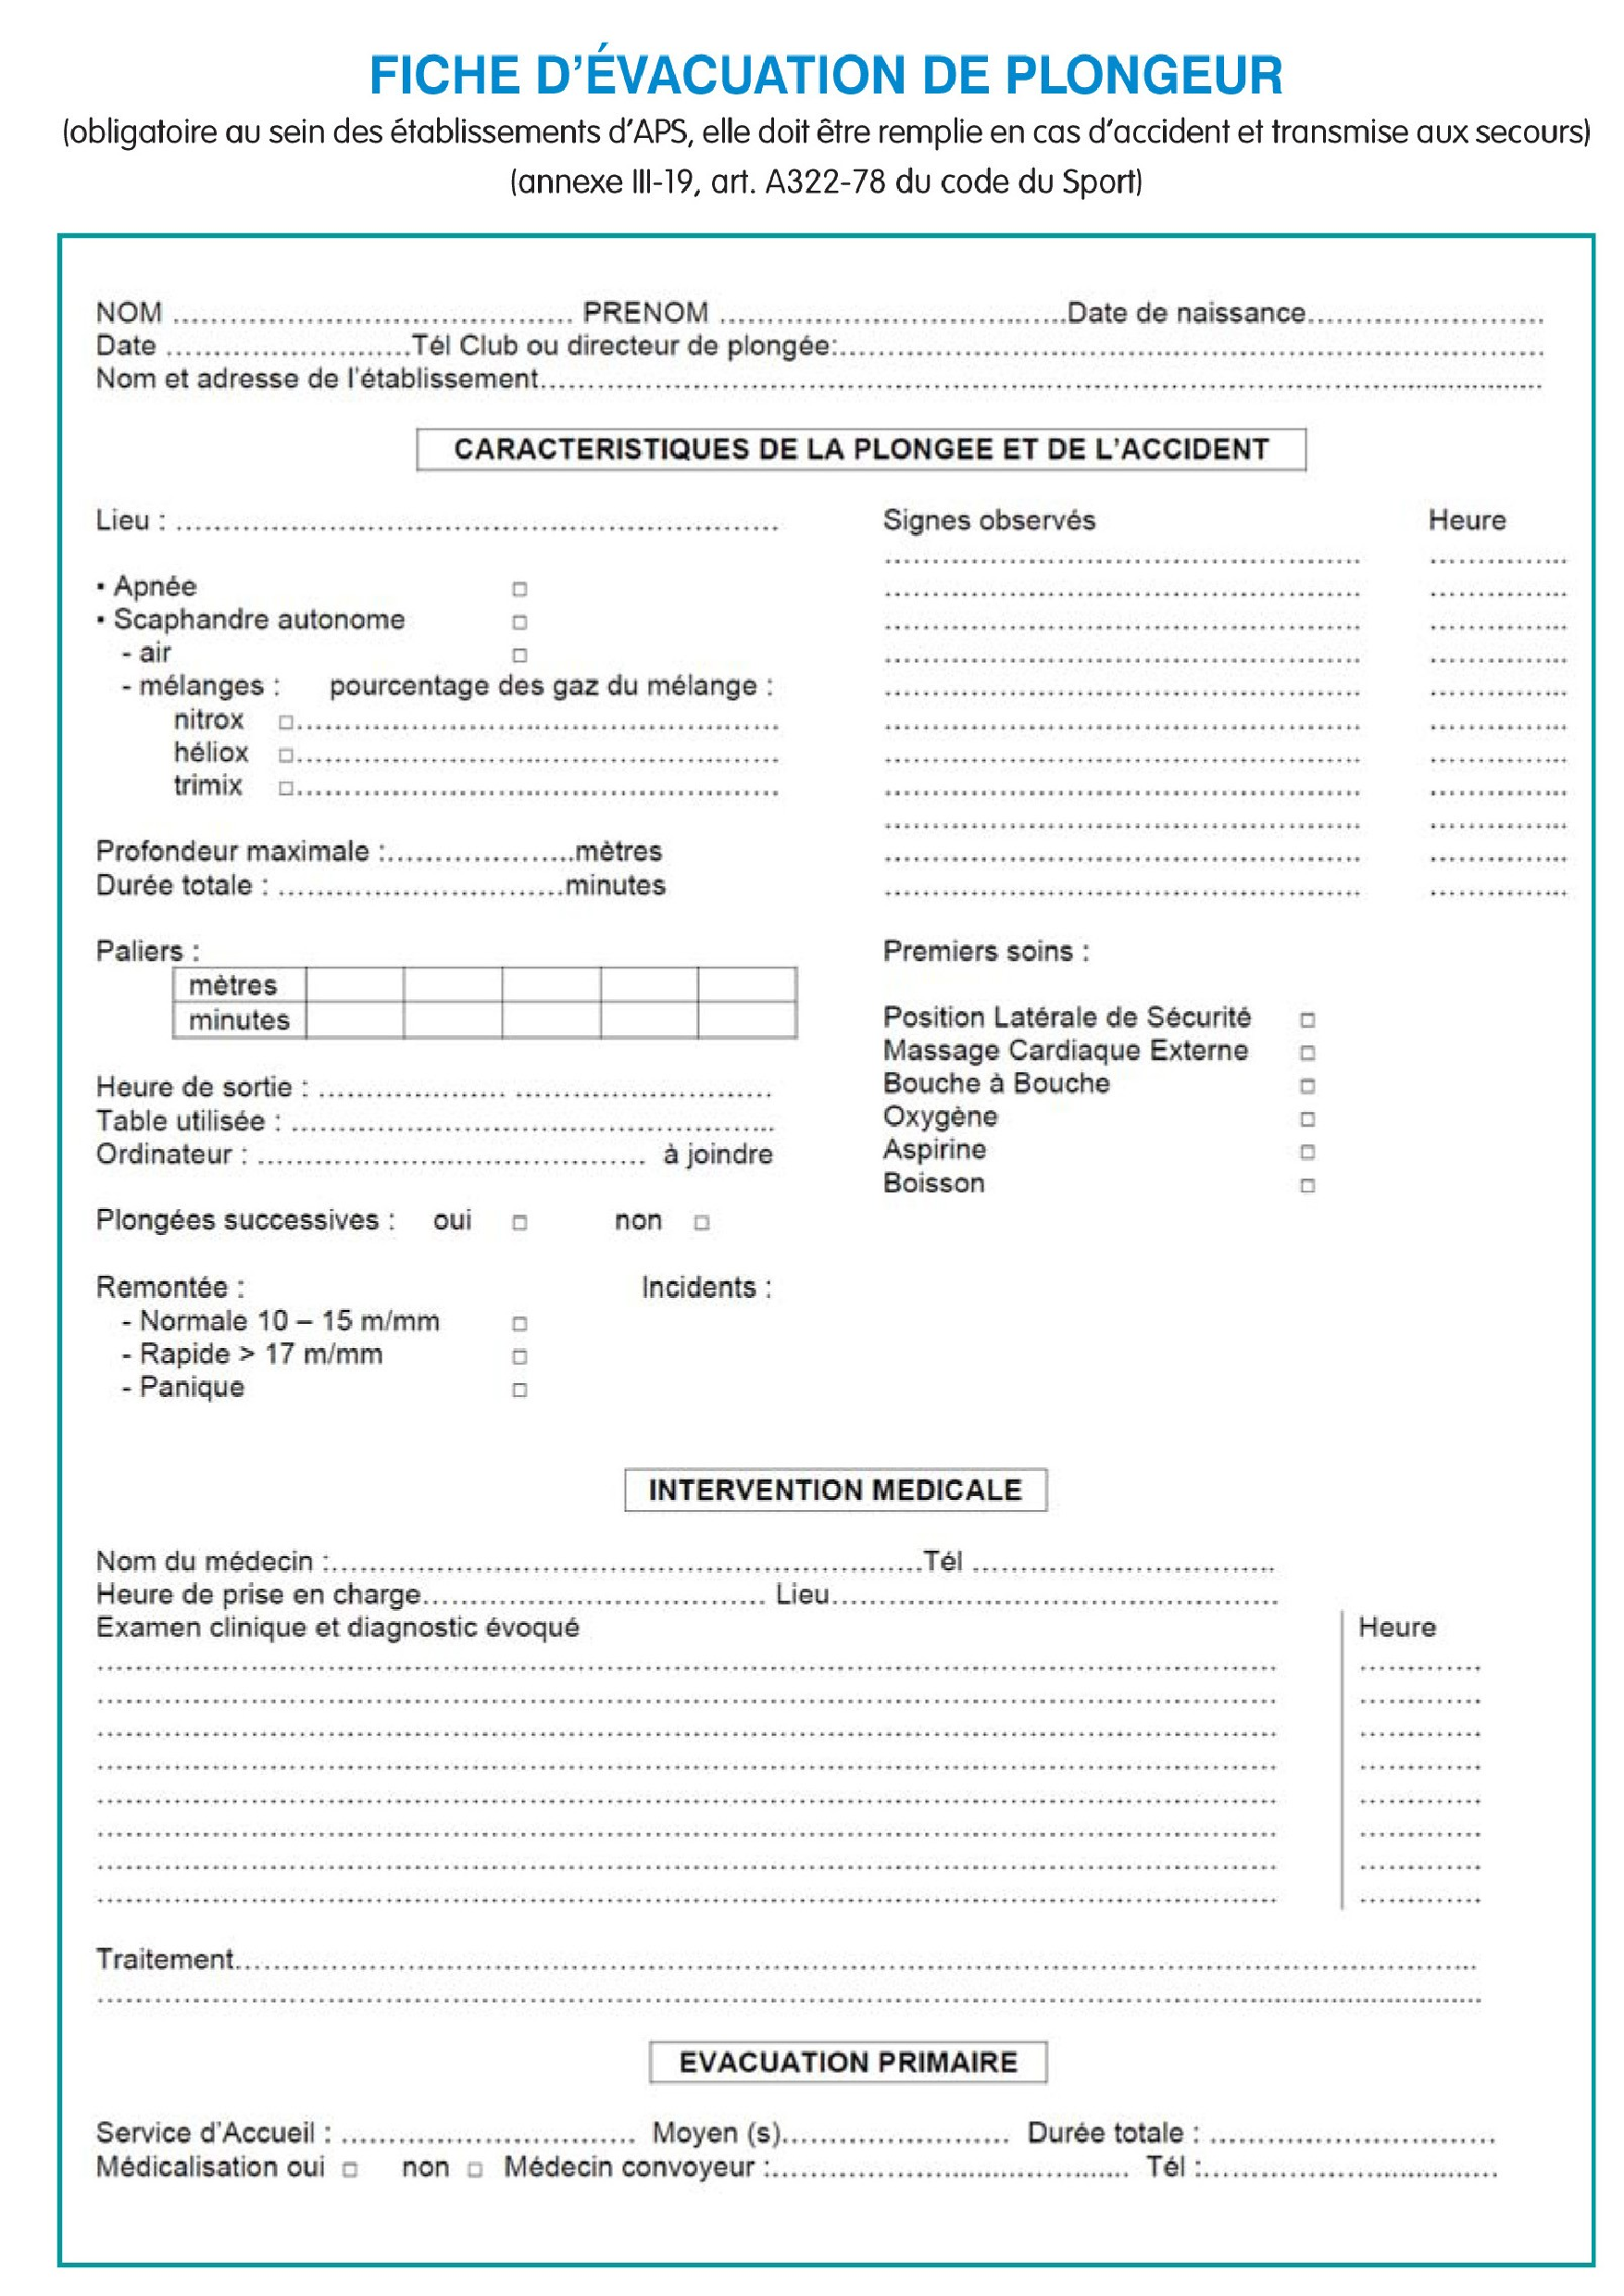
\includegraphics[height=0.85\textheight, keepaspectratio]{resources/pdf/fiche_d_evacuation.pdf}
\end{frame}

\begin{frame}{Organiser les Mises à l'Eau}
    \textbf{Logistique}
    \begin{itemize}
        \item Adapter le mouillage au profil (éviter si roches profondes ou houle).
    \end{itemize}

    \begin{alertblock}{Sécurité de Surface (Impératif)}
        \begin{itemize}
            \item \textbf{Pilote à bord} : Une personne compétente reste en surface.
            \item \textbf{Alternative} : Plongée \textbf{« en décalé »} (une palanquée assure la sécu pendant que l'autre plonge).
        \end{itemize}
    \end{alertblock}

    \vspace{0.5em}
    \textbf{Avant l'immersion}
    \begin{itemize}
        \item Remplir la \textbf{Fiche de Sécurité} (Noms, Aptitudes, Paramètres).
        \item \textbf{Vérification mutuelle} : Connaître l'équipement du binôme.
    \end{itemize}
\end{frame}

\begin{frame}{Fiche de Sécurité}
    \centering
    % Fiche de sécurité obligatoire pour le DP/Responsable
    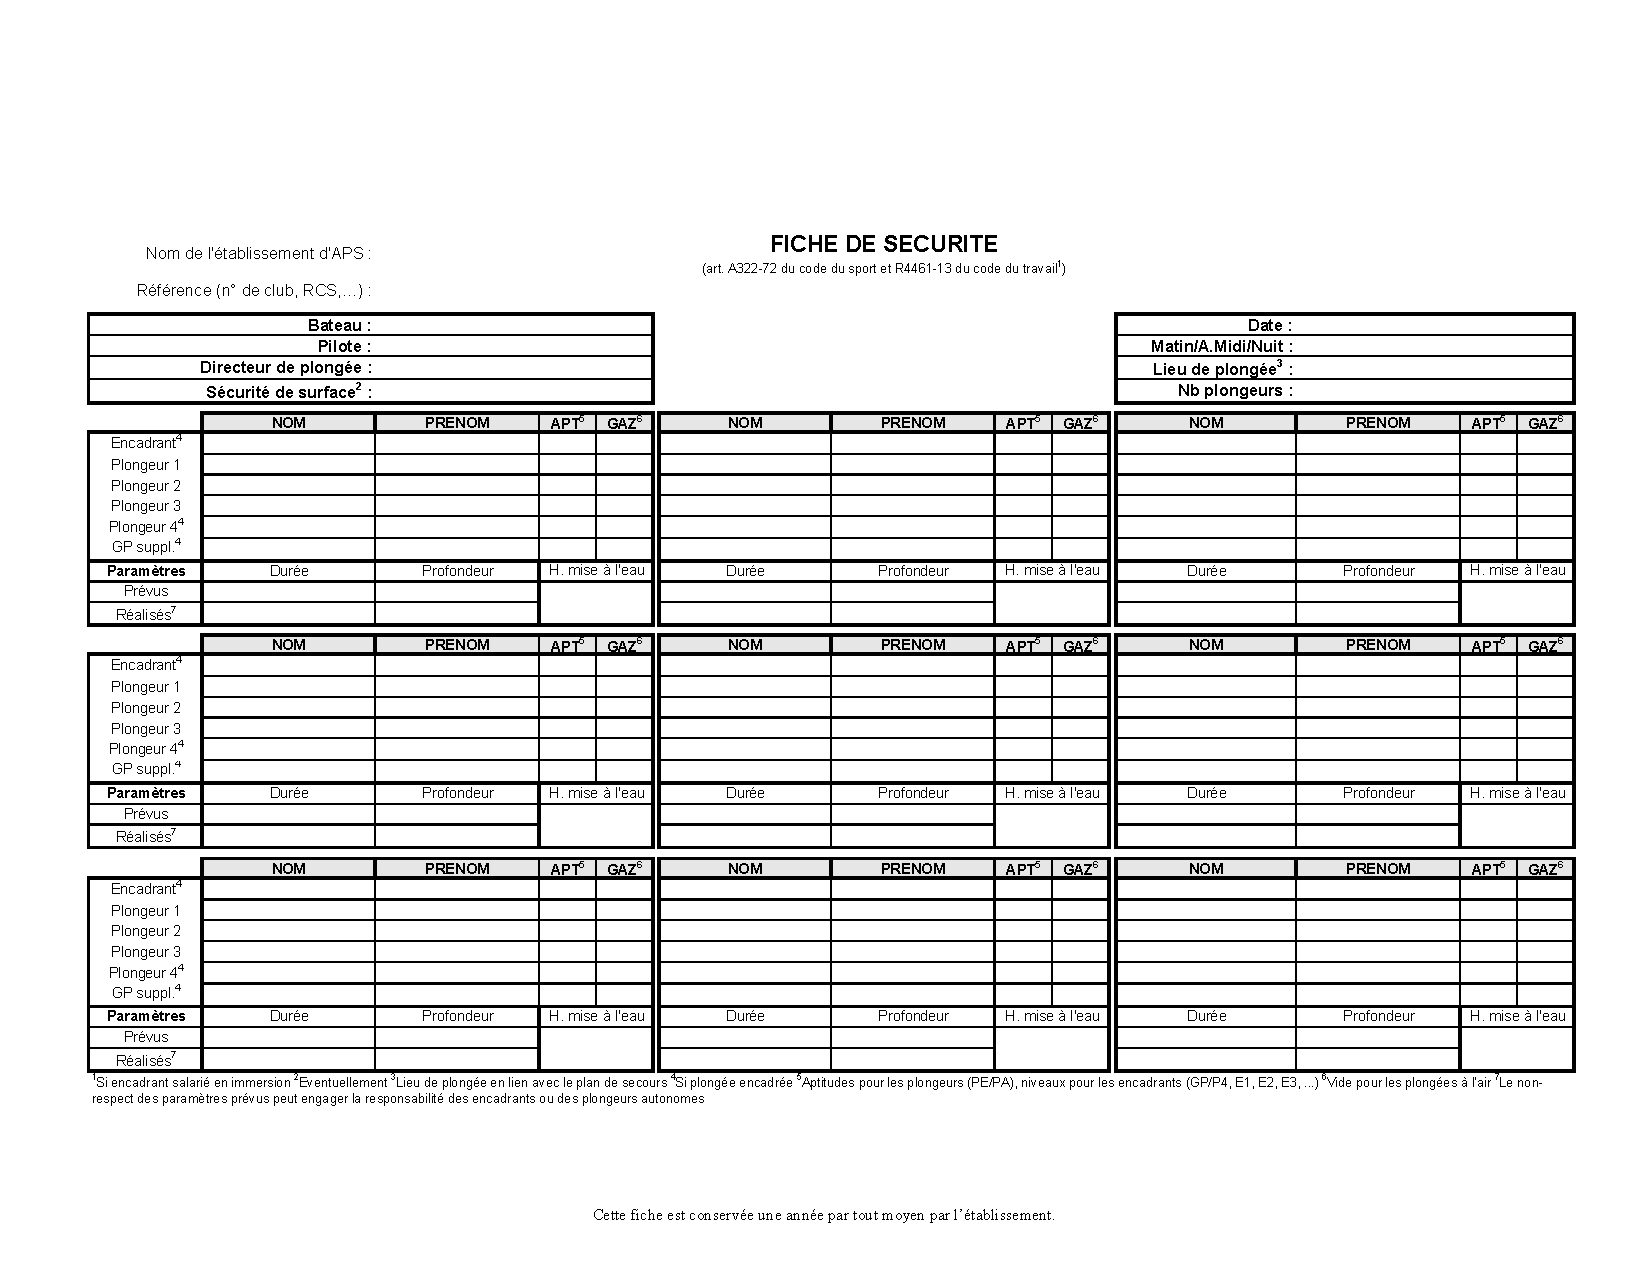
\includegraphics[height=\textheight, keepaspectratio,trim={0 0 0 3.9cm}, clip]{resources/pdf/fiche_de_securite.pdf}
\end{frame}

\begin{frame}{Matelotage — Nœuds utiles}
    \textbf{Savoir nouer est essentiel en bateau :}
    
    \vspace{0.5em}
    \begin{columns}[T,totalwidth=\textwidth]
        \column{0.5\textwidth}
        \textbf{Nœud de Chaise}
        \begin{itemize}
            \item Boucle fixe qui ne glisse pas.
            \item Idéal pour s'amarrer sur un anneau ou hisser du matériel.
        \end{itemize}
        \centering
        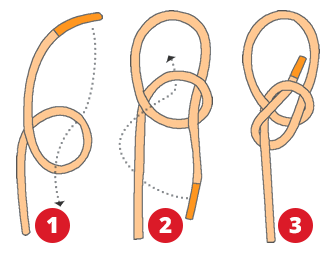
\includegraphics[height=0.4\textheight, keepaspectratio]{images/noeud-chaise.png}

        \column{0.5\textwidth}
        \textbf{Nœud de Cabestan}
        \begin{itemize}
            \item Nœud d'accroche rapide.
            \item Pour amarrer temporairement (autobloquant sous tension).
        \end{itemize}
        \centering
        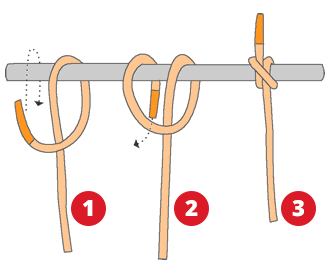
\includegraphics[height=0.4\textheight, keepaspectratio]{images/cabestan.png}
    \end{columns}
\end{frame}

\begin{frame}{Planification de la Palanquée}
    Avant la mise à l'eau, la palanquée doit se mettre d'accord sur:
    \begin{itemize}
        \item La \textbf{Profondeur Maximum}.
        \item La \textbf{Durée Maximum} (ou DTR max).
        \item La pression de décollage (réserve d'air).
        \item Le protocole de décompression (quel ordinateur suit-on ?).
        \item Les signes de communication spécifiques.
    \end{itemize}
    
    \begin{center}
        \textit{Plonger en autonomie, c'est plonger responsable !}
    \end{center}
\end{frame}